\section{Durchführung}
\label{sec:Durchführung}

\subsection{Bestimmung des Elastizitätsmoduls über die einseitige Einspannung}

Sowohl ein zylindrischer, als auch ein quaderförmiger Stab werden zunächst vermessen und gewogen.
Anschließend werden die Stäbe nacheinander einseitig, wie in Abbildung \ref{fig:durchfuehrung1} 
zu sehen ist, in die Vorrichtung eingespannt. 

\begin{figure}[H]
    \centering
    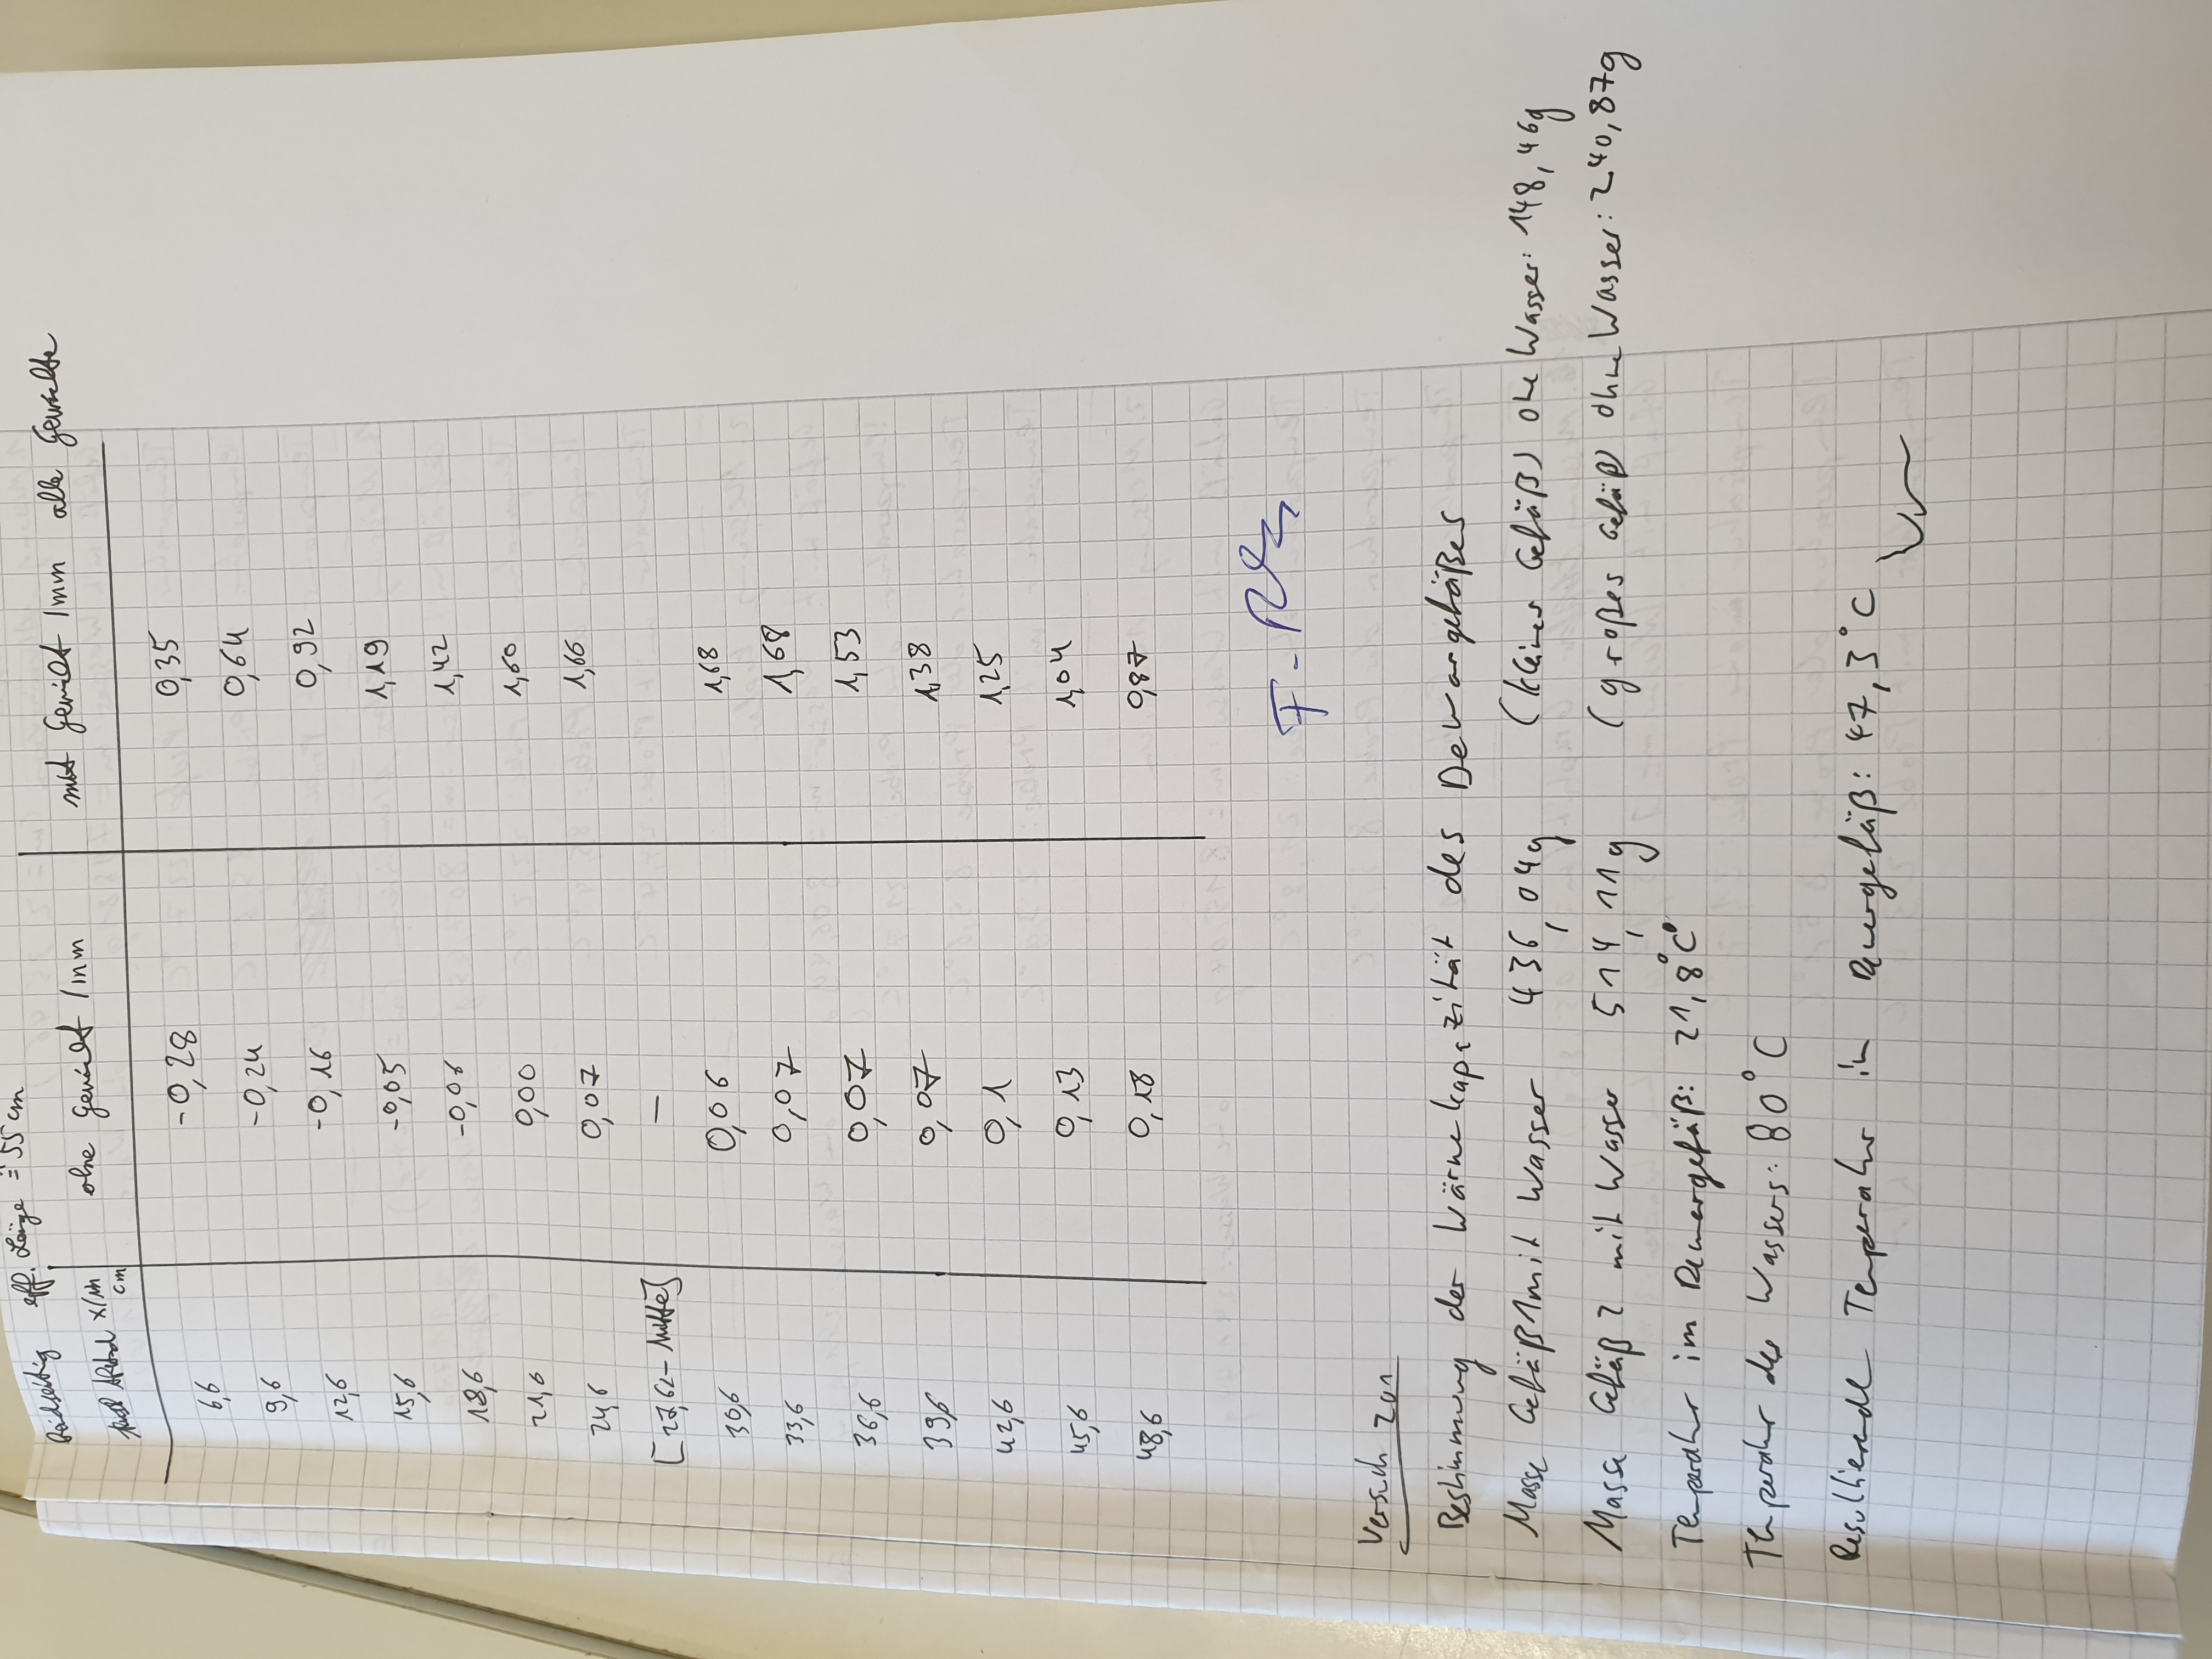
\includegraphics[width=10cm]{1.jpg}
    \caption{Aufbau zur einseitigen Messung der Durchbiegung ohne Gewicht}
    \label{fig:durchfuehrung1}
\end{figure}
\noindent
Nun soll die Auslenkung $D(x)$ ohne Verwendung eines Gewichts in 
Abhängigkeit von $x$ gemessen werden, wobei 15 Messwerte aufzunehmen sind. Daran angeschlossen
wird eine Masse $m_{Zylinder,1} = 503,2\, \si{\gram}$ beziehungsweise 
$m_{Rechteck,1} = 1168,8\, \si{\gram}$ über eine Aufhängung ($m_{A} = 40,4\, \si{\gram}$) 
an die Seite des Stabes gehangen (siehe Abbildung \ref{fig:durchfuehrung2}), welche 
nicht eingespannt wurde. Auch hier werden 15 Messwerte für die Auslenkung $D(x)$ in 
Abhängigkeit von $x$ aufgenommen. 

\begin{figure}[H]
    \centering
    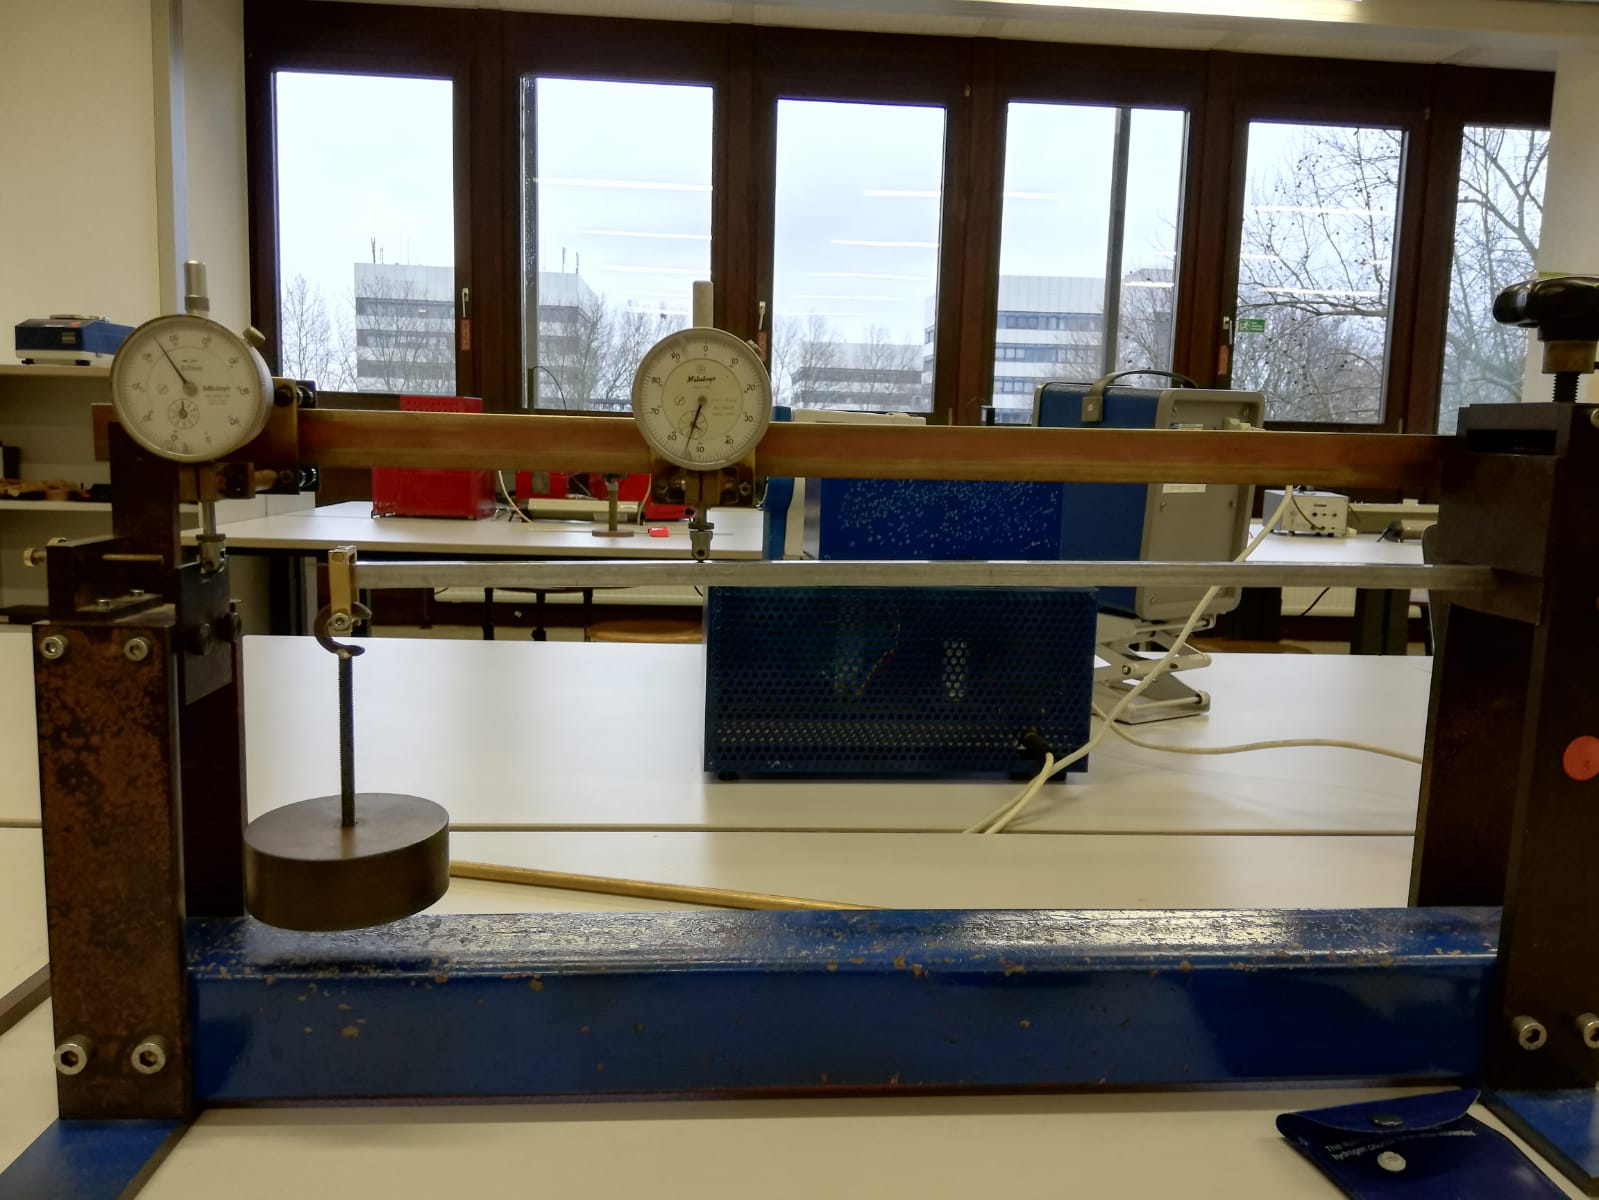
\includegraphics[width=10cm]{2.jpg}
    \caption{Aufbau zur Messung einseitigen Messung der Durchbiegung mit Gewicht}
    \label{fig:durchfuehrung2}
\end{figure}
\noindent


\subsection{Bestimmung des Elastizitätsmoduls über die beidseitige Einspannung}

Ähnlich wie beim ersten Teilversuch soll der Elastizitätsmoduls der beiden zuvor verwendeten 
Stäbe ermittelt werden. Zuerst wird jeweils ein Stab an beiden seiner Enden in der Vorrichtung 
eingespannt, wie in Abbildung \ref{fig:durchfuehrung3} zu sehen ist.
Hier sollen 15 Messwerte aufgenommen werden, welche die Abhängigkeit der Auslenkung $D(x)$ in 
Abhängigkeit von $x$ angeben. 

\begin{figure}[H]
    \centering
    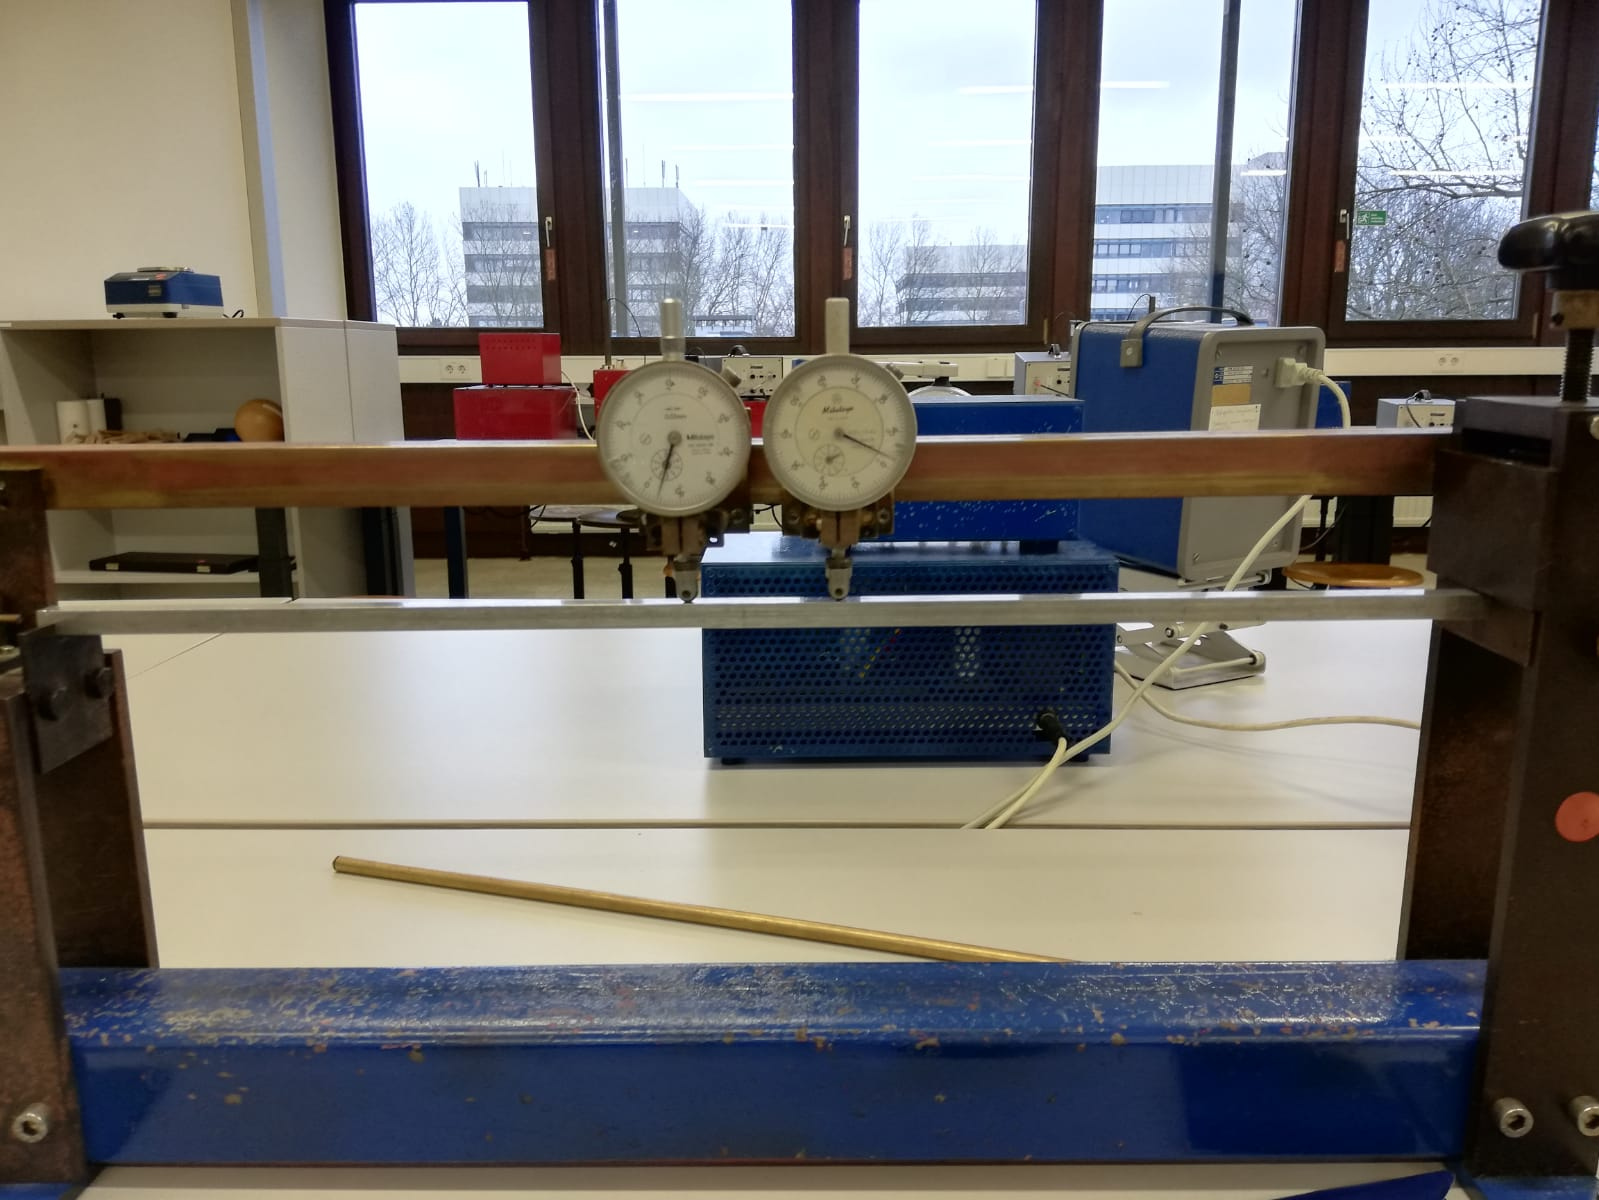
\includegraphics[width=10cm]{3.jpg}
    \caption{Aufbau zur beidseitigen Messung der Durchbiegung ohne Gewicht}
    \label{fig:durchfuehrung3}
\end{figure}
\noindent
Daran angeschlossen wird an die Mitte des Stabes ein Gewicht
aufgehangen und abermals soll die Auslenkung $D(x)$ abhängig von $x$ über 15 Messwerte
ermittelt werden. Hierbei beträgt die Masse des Gewichts $m_{2} = 2830,8\, \si{\gram}$. Auch in diesem 
Teil des Versuchs wurde die Aufhängung mit der Masse $m_{A} = 40,4\, \si{\gram}$ verwendet.
Dies lässt sich Abbildung \ref{fig:durchfuehrung4} entnehmen.

\begin{figure}[H]
    \centering
    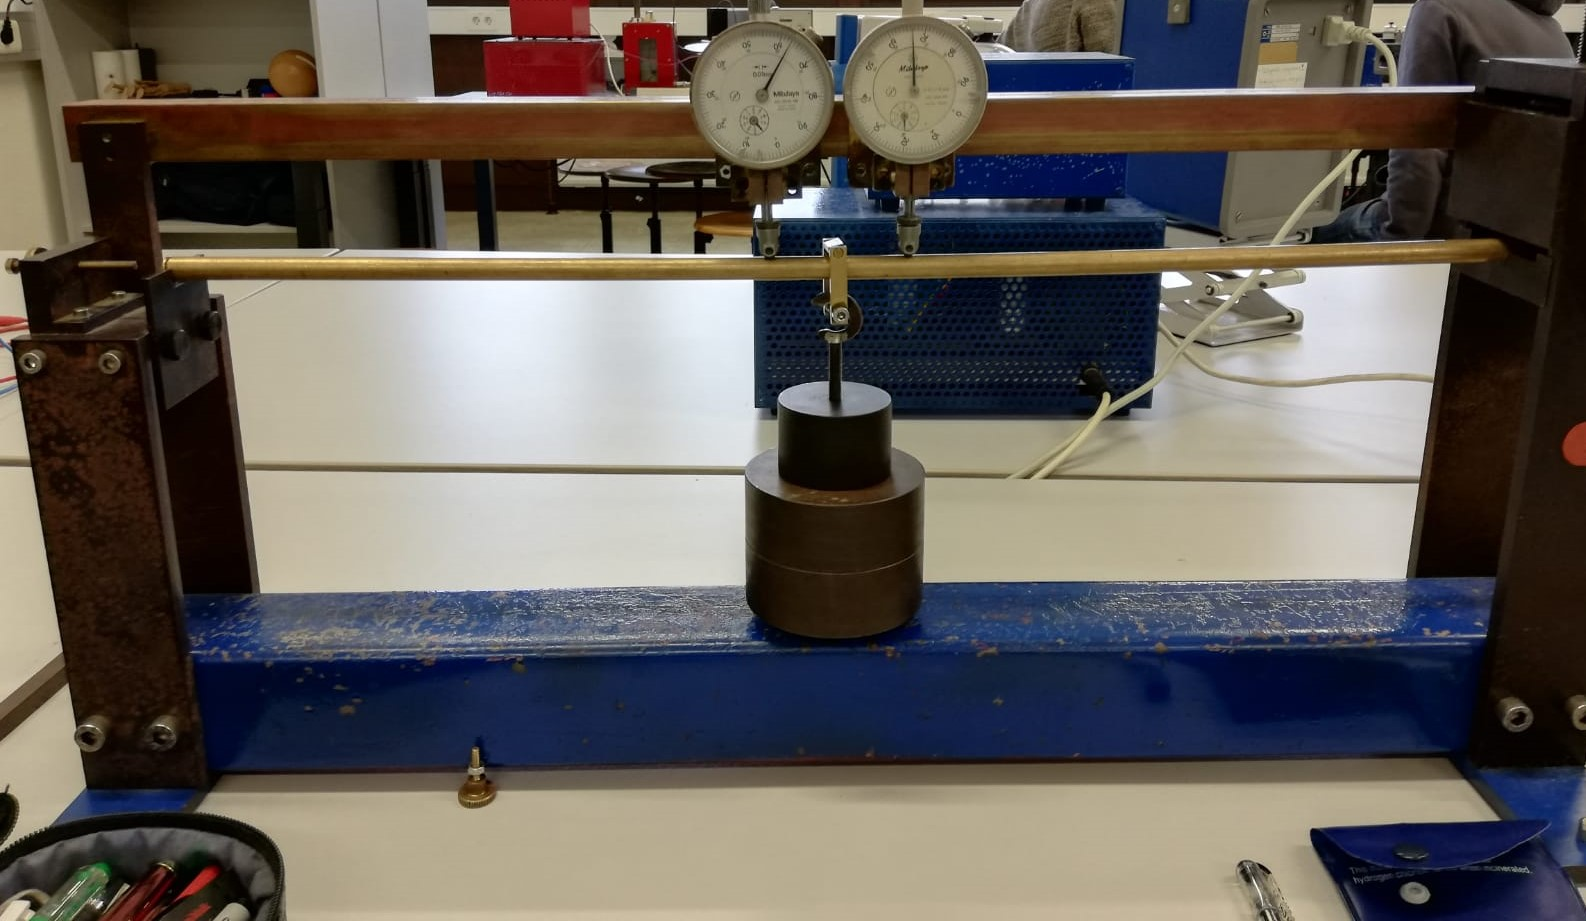
\includegraphics[width=10cm]{4.jpg}
    \caption{Aufbau zur beidseitigen Messung der Durchbiegung mit Gewicht}
    \label{fig:durchfuehrung4}
\end{figure}
